\documentclass[12pt, a4paper, openany]{report}

 % Encoding and Language
 \usepackage[utf8]{inputenc}
 \usepackage[T5,T1]{fontenc}
 \usepackage[english]{babel} % Changed from vietnamese to english

 % Mathematics
 \usepackage{amsmath}
 \usepackage{amsfonts}
 \usepackage{amssymb}

 % Graphics and Images
 \usepackage{graphicx}
 \usepackage{float}
 \usepackage{pdflscape}

 % Tables
 \usepackage{booktabs}
 \usepackage{longtable}
 \usepackage{array}

 % Text Formatting and Layout
 \usepackage{geometry}
 \usepackage{setspace}
 \usepackage{multicol}
 % \usepackage{times} % Times New Roman Font - DISABLED
 \usepackage{sectsty}
 \usepackage{enumitem}
 \usepackage{caption}
 \usepackage{microtype}

 % Code highlighting
 \usepackage{minted}

 % Hyperlinks and URL
 \usepackage{hyperref}
 \usepackage{xurl}

 % Bibliography
 \usepackage{natbib}

 % Others
 \usepackage{background}
 \usepackage{xcolor}
 \usepackage{indentfirst}
 \setlength{\parskip}{6pt plus 2pt minus 2pt}

 % --- Specific settings ---

 \onehalfspacing

 \chapterfont{\fontsize{20}{24}\selectfont\bfseries}
 \sectionfont{\fontsize{16}{20}\selectfont\bfseries}
 \subsectionfont{\fontsize{14}{18}\selectfont\bfseries}
 \subsubsectionfont{\fontsize{12}{15}\selectfont\bfseries}

 \captionsetup{labelfont=bf, skip=10pt}

 \definecolor{codebg}{rgb}{0.95,0.95,0.95}
 \setminted{
     bgcolor=codebg,
     fontsize=\footnotesize,
     linenos,
     frame=lines,
     framesep=2mm,
     breaklines,
     autogobble,
     python3=true,
     breaksymbolleft={}
 }

 \hypersetup{
     colorlinks=true,
     linkcolor=black,
     citecolor=black,
     urlcolor=black,
     filecolor=magenta,
     pdftitle={Image Classification on the CIFAR-10 Dataset using Convolutional Neural Network (CNN)}, % Translated
     pdfauthor={User}, % Translated (or keep as is if "Người dùng" is a specific name)
     bookmarksnumbered=true,
     unicode=true
 }

 \urlstyle{same}

 \backgroundsetup{
     scale=1,
     color=black,
     opacity=1,
     angle=0,
     position=current page.center,
     contents={
\includegraphics[width=\paperwidth,height=\paperheight]{background.png}}
 }

 \geometry{a4paper, margin=1in}

 % \setlist[itemize]{itemsep=2pt}

 \begin{document}

 % ----- Cover Page -----
 \begin{titlepage}
\BgThispage
    \centering
    \textbf{\large POSTS AND TELECOMMUNICATIONS INSTITUTE OF TECHNOLOGY}\\
    \textbf{\large FACULTY OF INFORMATION TECHNOLOGY I}
    \centerline{--------------------o0o--------------------}
    \vspace{1cm}
    
\includegraphics[width=8cm]{logo.png}\\ 
    \vspace{1cm}
{\Large \textbf{ASSIGNMENT REPORT 2}}\\[0.5cm]
{\LARGE \textbf{PYTHON PROGRAMMING LANGUAGE}}\\
\vfill
\begin{center}
\begin{tabular}{@{}l@{\hspace{2cm}}l}
\textbf{Instructor:}       & Kim Ngoc Bach \\
\textbf{Student:}          & Vu Thi Thu Duyen \\
\textbf{Student ID:}       & B23DCCE027 \\
\textbf{Class:}            & D23CQCEO6-B \\
\textbf{Academic Year:}    & 2023 - 2028 \\
\textbf{Training System:}  & Full-time University \\
\end{tabular}
\end{center}
\vfill
    {\large Hanoi, 2025}
\end{titlepage}
 \backgroundsetup{contents={}}

 % ----- Comments Page -----
 \newgeometry{top=2.5cm,bottom=2cm,left=3cm,right=2cm}

 \begin{center}
     \vspace*{1cm}
     \Large\textbf{LECTURER'S COMMENTS} % Translated
     \vspace{0.7cm}
 \end{center}

 \dotfill \vspace{0.25cm} \par
 \dotfill \vspace{0.25cm} \par
 \dotfill \vspace{0.25cm} \par
 \dotfill \vspace{0.25cm} \par
 \dotfill \vspace{0.25cm} \par
 \dotfill \vspace{0.25cm} \par
 \dotfill \vspace{0.25cm} \par
 \dotfill \vspace{0.25cm} \par
 \dotfill \vspace{0.25cm} \par
 \dotfill \vspace{0.25cm} \par
 \dotfill
 \vspace{1.0cm}

 {\textbf{\large{Grade: }}} \hspace{1.0cm}\textbf{(In words:} \hspace{2.5cm}\textbf{)} % Translated
 \vspace{1.5cm}

 \begin{flushright}
    Hanoi, date \hspace{0.75cm} month \hspace{0.75cm} year 20...\hspace{0.75cm} % Translated
    
    {\textbf{\large{Lecturer }}} \hspace{2cm} \textcolor{white}{.} % Translated
 \end{flushright}
 \clearpage
 \restoregeometry

 % ----- Table of Contents, List of Figures -----
 \tableofcontents
 \cleardoublepage
 \listoffigures
 \cleardoublepage

 % ----- Main Title and Abstract of the report -----
 \title{\bfseries IMAGE CLASSIFICATION ON THE CIFAR-10 DATASET USING CONVOLUTIONAL NEURAL NETWORK (CNN)} % Translated
 \author{}
 \date{}
 \maketitle

 \begin{abstract}
 \noindent \textbf{Data Source:} CIFAR-10 dataset - \url{https://www.cs.toronto.edu/~kriz/cifar.html} \\ % Translated
 \textbf{Task:} % Translated
 \begin{itemize}
     \item Build a Convolutional Neural Network (CNN) with 3 convolutional layers. % Translated
     \item Perform image classification, including training, validation, and testing steps. % Translated
     \item Plot learning curves. % Translated
     \item Plot confusion matrix. % Translated
     \item Use PyTorch library. % Translated
 \end{itemize}
 \end{abstract}
 \clearpage

 % ----- Content Chapters -----
 \chapter{Library Selection} % Translated
 To efficiently build and train a CNN model for image classification, I need libraries that support flexible tensor computations (prioritizing GPU but with CPU fallback), readily available network layers, optimization algorithms, image data processing, and results visualization.
 I chose the following libraries based on their ability to meet these requirements:
 \begin{itemize}
     \item \texttt{PyTorch (torch, torchvision)}: The core framework providing tensor structures with the ability to automatically detect and use GPUs when available, falling back to CPU when necessary. % Translated
     \item \texttt{torch.nn} \& \texttt{torch.optim}: Network layers (\texttt{Conv2d}, \texttt{Linear}, \texttt{BatchNorm2d}) and optimization algorithms (\texttt{AdamW}, \texttt{ReduceLROnPlateau}). % Translated
     \item \texttt{torchvision.transforms}: Tools for preprocessing and augmenting image data (\texttt{Normalize}, \texttt{RandomCrop}, \texttt{RandomHorizontalFlip}). % Translated
     \item \texttt{matplotlib} \& \texttt{seaborn}: Visualization of learning curves and confusion matrices. % Translated
     \item \texttt{numpy} \& \texttt{sklearn}: Data handling and confusion matrix calculation. % Translated
     \item \texttt{time} \& \texttt{os}: Measuring execution time and managing the file system. % Translated
     \item \texttt{multiprocessing}: Optimizing data loading. % Translated
 \end{itemize}

 \chapter{Methodology} % Translated
 \section{Data Preprocessing \& Augmentation} % Translated
 The initial phase focuses on preparing input data from the CIFAR-10 dataset. Images of size 32×32 pixels with 3 color channels are normalized to ensure stability during the learning process. I applied data augmentation techniques including random crop, horizontal flip, and random erasing of an image region. These augmentation methods help the model learn invariant features and reduce overfitting. % Translated

 \section{CNN Architecture with 3 Convolutional Layers} % Translated
 I constructed a CNN with 3 convolutional layers as per the problem requirements. After preprocessing, the image data is passed through a series of hierarchical convolutional layers. Each convolutional layer is combined with a ReLU activation function and a Pooling layer to form a complete processing unit. This architecture is designed to extract features hierarchically, from low-level features like edges and corners to more complex features like object parts and overall shapes. To enhance stability and optimize learning speed, I integrated Batch Normalization layers into the network architecture. % Translated

 \section{Classification and Output Layer} % Translated
 In the classification stage, features extracted from the 3 convolutional layers are converted into a one-dimensional vector through a flattening process. This feature vector is processed through Fully Connected layers to perform the final classification. To enhance generalization, I integrated a Dropout layer to control and reduce the risk of overfitting. The final output layer returns a probability distribution of predictions for the 10 object classes in the CIFAR-10 dataset. % Translated

 \section{Training and Evaluation} % Translated
 The training process is performed by optimizing the \texttt{CrossEntropyLoss} function combined with the Label Smoothing technique, using the \texttt{AdamW} optimization algorithm. I train on the training set, monitor performance on the validation set, and perform final evaluation on the test set. % Translated

 \section{Visualization and Result Analysis} % Translated
 To evaluate performance and analyze the model's results in detail, I use two main visualization methods:
 \begin{itemize}
     \item Learning Curves: Plotting loss and accuracy curves on the training and validation sets to monitor the training process and detect overfitting. % Translated
     \item Confusion Matrix: Creating a confusion matrix to analyze classification performance on each object class and identify classes that are often confused. % Translated
 \end{itemize}

 \chapter{Implementation Process} % Translated
 \section{Configuration} % Translated
 The deep learning model training process depends on many hyperparameters and environmental settings. I need to centrally manage configurations to ensure flexibility, result reproducibility, and maximum utilization of hardware resources. I define the main configurations including:
 \begin{itemize}
     \item \textbf{Hardware Configuration:} % Translated
     \begin{itemize}
         \item \texttt{DEVICE}: Automatically detects GPU (\texttt{cuda:0}) or CPU % Translated
         \item \texttt{PIN\_MEMORY}: Automatically enabled with GPU to optimize data transfer % Translated
         \item \texttt{NUM\_WORKERS = 2}: Number of parallel processes for data loading % Translated
     \end{itemize}
     \item \textbf{Training Hyperparameters:} % Translated
     \begin{itemize}
         \item \texttt{BATCH\_SIZE = 128}: Batch size balancing efficiency and memory % Translated
         \item \texttt{LEARNING\_RATE = 0.001}: Initial learning rate for AdamW % Translated
         \item \texttt{WEIGHT\_DECAY = 5e-4}: Increased L2 regularization to combat overfitting % Translated
         \item \texttt{NUM\_EPOCHS\_INITIAL = 300}: Maximum number of epochs allowed % Translated
         \item \texttt{VALIDATION\_SPLIT = 0.2}: 20\% of training data reserved for validation % Translated
     \end{itemize}
     \item \textbf{Adjustment and Early Stopping Mechanisms:} % Translated
     \begin{itemize}
         \item \texttt{EARLY\_STOP\_PATIENCE = 5}: Early stopping after 5 epochs with no improvement in validation loss % Translated
         \item \texttt{LR\_SCHEDULER\_PATIENCE = 3}: Reduce learning rate after 3 epochs with no improvement % Translated
     \end{itemize}
     \item \textbf{Regularization Techniques:} % Translated
     \begin{itemize}
         \item \texttt{DROPOUT\_RATE = 0.5}: High dropout rate to prevent overfitting % Translated
         \item \texttt{LABEL\_SMOOTHING\_FACTOR = 0.1}: Label smoothing improves generalization % Translated
     \end{itemize}
     \item \textbf{Reproducibility:} % Translated
     \begin{itemize}
         \item \texttt{SEED = 42}: Fixed seed ensures consistent results across runs % Translated
     \end{itemize}
 \end{itemize}

 \section{Data Transforms} % Translated
 Raw image data presents several problems when fed directly into a neural network model. The first issue is incompatible format – PyTorch neural networks require input to be Tensors, while original images are in PIL or NumPy array format.

 Besides, unnormalized pixel value scales also create difficulties during training. Pixel values typically range from [0, 255], which is too large for optimal processing by neural networks. Normalizing to a smaller range like [0,1] or [-1,1] helps the training process become more stable and converge faster.

 Another important issue is the lack of diversity in the training set. Since the training set has a finite size, if the model only learns from the original samples, it can easily overfit the training data and perform poorly on new, unseen data. Therefore, augmentation techniques are needed to create diversity for the training data.

 Furthermore, it's necessary to clearly distinguish between the training and evaluation phases. Random transformations for data augmentation should only be applied to the training set, not to the validation and test sets, to ensure that evaluation is consistent and objective.

 To address the issues mentioned above, I design separate transformations for the training set (\texttt{TRANSFORM\_TRAIN}) and the validation/test set (\texttt{TRANSFORM\_VAL\_TEST}) using \texttt{transforms.Compose} to create a sequential processing pipeline.

 \subsection{\texttt{TRANSFORM\_TRAIN} - Transforms for the Training Set} % Translated
 This pipeline both prepares the data format and enhances diversity. I start with \texttt{transforms.RandomCrop(32, padding=4)} - padding 4 pixels on each side then randomly cropping a 32x32 pixel region. This helps the model learn to recognize objects in different positions and become less sensitive to translations.

 Next, \texttt{transforms.RandomHorizontalFlip()} flips the image horizontally with a 50\% probability. This technique is effective for CIFAR-10 because horizontally flipping objects like cars or dogs does not change their meaning.

 \texttt{transforms.ToTensor()} plays a key role, converting images from PIL/NumPy to PyTorch Tensors and automatically normalizing pixel values from [0, 255] to [0.0, 1.0]. This order is important because subsequent steps require Tensor input. \texttt{transforms.RandomErasing(p=0.3, scale=(0.02, 0.2), ratio=(0.3, 3.3))} with a 30\% probability will randomly erase a rectangular region in the image. The size of the erased region ranges from 2-20\% of the image area, with an aspect ratio from 0.3-3.3. This technique forces the model to learn from different parts of the object, increasing its robustness to occlusions.

 Finally, \texttt{transforms.Normalize((0.5, 0.5, 0.5), (0.5, 0.5, 0.5))} normalizes each color channel to the range [-1.0, 1.0] using the calculation \texttt{(pixel - 0.5) / 0.5}. This normalization helps the training process become more stable and converge faster.

 \begin{minted}{python}
 TRANSFORM_TRAIN = transforms.Compose([
     transforms.RandomCrop(32, padding=4),
     transforms.RandomHorizontalFlip(),
     transforms.ToTensor(),
     transforms.RandomErasing(p=0.3, scale=(0.02, 0.2), ratio=(0.3, 3.3), value='random'),
     transforms.Normalize((0.5, 0.5, 0.5), (0.5, 0.5, 0.5))
 ])
 \end{minted}

 \subsection{\texttt{TRANSFORM\_VAL\_TEST} - Transforms for Validation and Test Sets} % Translated
 This pipeline only prepares the data format without altering the nature of the images for objective evaluation. I only use \texttt{transforms.ToTensor()} to convert to Tensor and normalize to [0.0, 1.0], followed by \texttt{transforms.Normalize((0.5, 0.5, 0.5), (0.5, 0.5, 0.5))} to normalize to [-1.0, 1.0].

 Random augmentation operations like \texttt{RandomCrop}, \texttt{RandomHorizontalFlip}, \texttt{RandomErasing} are not applied at all. The purpose is to evaluate the true performance of the model on "clean" data, ensuring the consistency and objectivity of the evaluation results.

 \begin{minted}{python}
 TRANSFORM_VAL_TEST = transforms.Compose([
     transforms.ToTensor(),
     transforms.Normalize((0.5, 0.5, 0.5), (0.5, 0.5, 0.5))
 ])
 \end{minted}

 \section{Model Definition - Net} % Translated
 The model I designed follows the principle of balancing representational power and practicality. The architecture is deep enough to learn complex features but not overly complex to avoid overfitting and excessive resource consumption. Each component in the architecture has a specific role: \texttt{BatchNorm} helps stabilize training, \texttt{MaxPool} creates invariance and reduces computation, \texttt{Dropout} prevents overfitting, and the hierarchical structure ensures efficient feature learning from basic to complex. This design is suitable for basic to intermediate image classification tasks with good scalability.

 \subsection{Overall Structure} % Translated
 The \texttt{Net} class inherits from \texttt{nn.Module} and includes two main parts: three convolutional blocks for feature extraction and two fully connected layers for classification. I designed it with the principle of gradually increasing the number of channels from 3 to 32, 64, then 128 channels, while simultaneously reducing the spatial dimensions from 32×32 to 16×16, 8×8, and finally 4×4. This principle helps the network learn features from simple to complex in a natural way.

 \subsection{Convolutional Blocks} % Translated
 The first convolutional block \texttt{conv1} takes a 3-channel RGB image as input and produces 32 feature maps with a 3×3 kernel and \texttt{padding=1} to preserve the image size. The normalization layer \texttt{bn1} is applied immediately after to normalize the data distribution, helping to stabilize the training process and accelerate learning. The pooling layer \texttt{pool1} with a 2×2 size halves the image dimensions, creating translation invariance and reducing computational load.

 The second block has a similar structure but increases the number of channels from 32 to 64 to learn more complex features from the output of the first block. This increase in channels allows the network to represent many different types of intermediate-level features.

 The third block further increases to 128 channels to learn the highest-level features. After three pooling operations, the original 32×32 pixel image is reduced to 4×4 pixels.

 The gradual increase in the number of channels in this architecture has profound significance. In the first block, the network only needs to learn basic features like edges and corners, so 32 channels are sufficient. In the middle block, the network needs to combine edges to form more complex shapes, thus requiring 64 channels. In the final block, the network must learn high-level features like textures and patterns, so it needs 128 channels. This design allows the network to learn systematically and optimize computational resources.

 \begin{minted}{python}
 self.conv1 = nn.Conv2d(3, 32, kernel_size=3, padding=1)
 self.bn1 = nn.BatchNorm2d(32)
 self.pool1 = nn.MaxPool2d(kernel_size=2, stride=2)

 self.conv2 = nn.Conv2d(32, 64, kernel_size=3, padding=1)
 self.bn2 = nn.BatchNorm2d(64)
 self.pool2 = nn.MaxPool2d(kernel_size=2, stride=2)

 self.conv3 = nn.Conv2d(64, 128, kernel_size=3, padding=1)
 self.bn3 = nn.BatchNorm2d(128)
 self.pool3 = nn.MaxPool2d(kernel_size=2, stride=2)
 \end{minted}

 \subsection{Classification Layers} % Translated
 After feature extraction, the output tensor of size \texttt{(batch\_size, 128, 4, 4)} is flattened to \texttt{(batch\_size, 2048)} to prepare for the fully connected layers. The first fully connected layer \texttt{fc1} transforms 2048 features down to 512 features, accompanied by a normalization layer \texttt{bn\_fc1} to stabilize learning.

 I apply dropout only in the fully connected layers because this is where the largest number of parameters exists, thus having the highest risk of overfitting. Convolutional layers, due to their weight-sharing mechanism, are less prone to overfitting. The final layer \texttt{fc2} generates logits for each classification class, with the number of outputs equal to \texttt{num\_classes}.

 \begin{minted}{python}
 self.fc1 = nn.Linear(128 * 4 * 4, 512)
 self.bn_fc1 = nn.BatchNorm1d(512)
 self.dropout = nn.Dropout(dropout_rate)
 self.fc2 = nn.Linear(512, num_classes)
 \end{minted}

 \subsection{Forward Pass} % Translated
 Data passes through three convolutional blocks following a fixed pattern: \texttt{Convolution -> BatchNorm -> ReLU -> MaxPool}, where I chose the ReLU activation function because it is computationally fast, simple, and helps avoid the vanishing gradient problem during training. After passing through the three feature extraction blocks, the data is flattened and passed through two fully connected layers with dropout applied in between to combat overfitting. The final output is a logit tensor that will be processed by the \texttt{CrossEntropyLoss} function, which already integrates Softmax to calculate probabilities and loss for the training process.

 \begin{minted}{python}
 def forward(self, x):
     x = self.pool1(F.relu(self.bn1(self.conv1(x))))
     x = self.pool2(F.relu(self.bn2(self.conv2(x))))
     x = self.pool3(F.relu(self.bn3(self.conv3(x))))
     x = x.view(-1, 128 * 4 * 4)
     x = F.relu(self.bn_fc1(self.fc1(x)))
     x = self.dropout(x)
     x = self.fc2(x)
     return x
 \end{minted}

 \section{Helper Functions} % Translated
 During the development of the deep learning training program, I noticed that many logic segments were repetitive or performed specific, independent tasks. This led to the code becoming lengthy and difficult to maintain. Specifically, three main issues needed addressing: loading and preprocessing data into batches, the process of executing a training epoch with fixed steps, and the process of evaluating the model on a dataset without updating weights.

 To solve these problems, I encapsulated these logic segments into separate helper functions. This approach makes the source code more modular, readable, and maintainable. At the same time, it allows for code reuse and makes the main execution function cleaner, focusing on overall coordination rather than implementation details.

 \subsection{Function \texttt{get\_dataloaders}: Preparing the Data Pipeline} % Translated
 Deep learning models require input data to be provided in a structured and efficient manner. Five main challenges need to be addressed. First is reliably loading data from the source. Next is splitting the original dataset into training and validation sets to monitor the learning process. Third is applying appropriate transformations for each dataset. Fourth is creating data batches for efficient processing on the GPU. Finally is shuffling the training data to reduce gradient variance and help the model converge better.

 To achieve optimal efficiency, I need to load and preprocess data in parallel with GPU computation. PyTorch's \texttt{DataLoader} combined with \texttt{Dataset} and \texttt{Sampler} is the optimal solution for these problems.

 \subsubsection*{Implementation Logic and Processing Flow} % Translated
 \noindent\textbf{Step 1: Ensure data is available} % Translated

 I start by downloading the CIFAR-10 data to the machine via the command \texttt{download=True}, the result is assigned to the variable "\_" because I only need to ensure the data exists and do not use it directly. Immediately after, I create \texttt{full\_train\_dataset} for actual work with \texttt{download=False}, avoiding unnecessary re-downloads. % Translated

 \noindent\textbf{Step 2: Random data splitting} % Translated

 I split the original training set into two parts: training and validation. First, I calculate the number of validation samples based on the defined ratio and use \texttt{np.floor} to ensure the result is an integer.
 The most important step is to create a list of indices from 0 to the total number of samples, then apply \texttt{np.random.shuffle} to randomly shuffle them. This shuffling ensures that validation samples are evenly distributed across the entire dataset, without bias. After shuffling, I split the list into \texttt{val\_idx} (the beginning part) and \texttt{train\_idx} (the remaining part). % Translated

 \noindent\textbf{Step 3: Apply appropriate transforms} % Translated

 Due to different processing requirements, I create two separate datasets from the same original data source. The dataset for training uses \texttt{TRANSFORM\_TRAIN}, which includes data augmentation like rotation, flipping, and color changes to increase diversity. The dataset for validation only applies \texttt{TRANSFORM\_VAL\_TEST} with basic normalization operations, without random augmentation, to ensure consistent evaluation results. % Translated

 \noindent\textbf{Step 4: Create samplers for selective sampling} % Translated

 I use \texttt{SubsetRandomSampler} to ensure that each dataset only takes the correctly allocated samples. \texttt{train\_sampler} only takes samples with indices in \texttt{train\_idx} and still maintains randomness in each epoch. \texttt{val\_sampler} operates similarly with \texttt{val\_idx}. % Translated

 \noindent\textbf{Step 5: Build complete DataLoaders} % Translated

 Finally, I create three \texttt{DataLoader} instances for different purposes. \texttt{trainloader} combines the augmented dataset with \texttt{train\_sampler}, ensuring only training samples are used with the appropriate transform. \texttt{valloader} does similarly with the normalized dataset and \texttt{val\_sampler}.

 \texttt{testloader} is created separately from the original CIFAR-10 test set with \texttt{train=False} and \texttt{shuffle=False} because order is not important in the final evaluation. All \texttt{DataLoader}s are optimized with \texttt{num\_workers} and \texttt{pin\_memory} for parallel processing and to speed up data transfer to the GPU.

 The result is a complete data pipeline: \texttt{trainloader} with augmentation for training, \texttt{valloader} with basic transforms for validation, and \texttt{testloader} for final evaluation.

 \begin{minted}{python}
 def get_dataloaders(batch_size, num_workers, pin_memory, validation_split):
     _ = torchvision.datasets.CIFAR10(root='./data', train=True, download=True)
     full_train_dataset = torchvision.datasets.CIFAR10(root='./data', train=True, download=False)

     num_train_val = len(full_train_dataset)
     indices = list(range(num_train_val))
     split = int(np.floor(validation_split * num_train_val))
     np.random.shuffle(indices)
     train_idx, val_idx = indices[split:], indices[:split]

     train_dataset = torchvision.datasets.CIFAR10(root='./data', train=True, transform=TRANSFORM_TRAIN, download=False)
     val_dataset = torchvision.datasets.CIFAR10(root='./data', train=True, transform=TRANSFORM_VAL_TEST, download=False)

     train_sampler = torch.utils.data.SubsetRandomSampler(train_idx)
     val_sampler = torch.utils.data.SubsetRandomSampler(val_idx)

     trainloader = torch.utils.data.DataLoader(train_dataset, batch_size=batch_size, sampler=train_sampler, num_workers=num_workers, pin_memory=pin_memory)
     valloader = torch.utils.data.DataLoader(val_dataset, batch_size=batch_size, sampler=val_sampler, num_workers=num_workers, pin_memory=pin_memory)

     test_dataset = torchvision.datasets.CIFAR10(root='./data', train=False, transform=TRANSFORM_VAL_TEST, download=True)
     testloader = torch.utils.data.DataLoader(test_dataset, batch_size=batch_size, shuffle=False, num_workers=num_workers, pin_memory=pin_memory)
     return trainloader, valloader, testloader
 \end{minted}

 \subsection{Function \texttt{train\_one\_epoch}: Perform a complete training epoch} % Translated
 This function is responsible for performing a full training pass over all data in \texttt{trainloader}, including updating model weights and tracking performance metrics. Below is the systematic logic for each step:

 \subsubsection*{Prepare the model and initialize tracking variables} % Translated
 I start by switching the model to training mode via \texttt{model.train()}, which is important because Dropout will be activated and \texttt{BatchNorm2d} will update its statistics based on the current data. Concurrently, I initialize variables \texttt{running\_loss}, \texttt{correct\_train}, and \texttt{total\_train} to track the overall performance of the epoch.

 \subsubsection*{Process each batch of data in a standard sequence of steps} % Translated
 For each batch from \texttt{trainloader}, I perform a four-step main process. First, move \texttt{inputs} and \texttt{labels} to the \texttt{device} for consistency. Next, call \texttt{optimizer.zero\_grad()} to clear gradients from the previous batch because PyTorch accumulates gradients by default.

 Then, I perform a forward pass through \texttt{outputs = model(inputs)} and calculate the loss using \texttt{loss = criterion(outputs, labels)}. Finally, \texttt{loss.backward()} computes gradients via backpropagation, and \texttt{optimizer.step()} updates the weights in the direction that minimizes the loss.

 \subsubsection*{Collect statistics and calculate accuracy} % Translated
 During processing, I continuously update tracking metrics. Loss is accumulated by multiplying \texttt{loss.item()} with the batch size to ensure accurate calculation when batches may differ in size.
 To evaluate accuracy, I use \texttt{torch.max(outputs.data, 1)} to find the class with the highest score as the prediction, then compare it with the actual labels to count the number of correct predictions and update the total number of samples.

 \subsubsection*{Calculate end-of-epoch results} % Translated
 Upon completing all batches, I calculate the average loss by dividing the total loss by the total number of samples, and accuracy as the percentage of correct predictions. The function returns \texttt{epoch\_loss} and \texttt{epoch\_acc} to provide an overview of the model's performance, while also checking \texttt{total\_train > 0} to avoid division by zero errors.

 \begin{minted}{python}
 def train_one_epoch(model, trainloader, criterion, optimizer, device):
     model.train()
     running_loss = 0.0
     correct_train = 0
     total_train = 0
     for inputs, labels in trainloader:
         inputs, labels = inputs.to(device), labels.to(device)
         optimizer.zero_grad()
         outputs = model(inputs)
         loss = criterion(outputs, labels)
         loss.backward()
         optimizer.step()
         running_loss += loss.item() * inputs.size(0)
         _, predicted = torch.max(outputs.data, 1)
         total_train += labels.size(0)
         correct_train += (predicted == labels).sum().item()
     epoch_loss = running_loss / total_train if total_train > 0 else 0.0
     epoch_acc = 100 * correct_train / total_train if total_train > 0 else 0.0
     return epoch_loss, epoch_acc
 \end{minted}

 \subsection{Function \texttt{validate\_one\_epoch(model, valloader, criterion, device)}} % Translated
 The \texttt{validate\_one\_epoch} function evaluates the model's performance on the validation set after each training epoch. This process not only helps monitor overfitting by comparing performance between the training and validation sets but also provides crucial information for adjusting hyperparameters like learning rate scheduling and early stopping. Additionally, the validation result is the basis for saving the best-performing model.

 \subsubsection*{Prepare the model for the evaluation process} % Translated
 Before starting the evaluation, I execute \texttt{model.eval()} to switch the model to evaluation mode. This changes the behavior of special layers: Dropout stops deactivating neurons, and BatchNorm uses running statistics instead of calculating them from the current batch. Then, I initialize tracking variables \texttt{running\_loss = 0.0}, \texttt{correct\_val = 0}, \texttt{total\_val = 0} to accumulate results throughout the evaluation process.

 \subsubsection*{Perform evaluation with \texttt{torch.no\_grad()}} % Translated
 I use \texttt{torch.no\_grad()} to create an environment that does not track gradients, which saves memory and speeds up processing. Within this block, I iterate through each batch from \texttt{valloader}, move the data to the appropriate \texttt{device}, and then perform a forward pass to get predictions. For each batch, I calculate the loss using \texttt{criterion} and accumulate it into \texttt{running\_loss}, while also using \texttt{torch.max()} to find the predicted class with the highest probability.

 \subsubsection*{Calculate and return results} % Translated
 To assess accuracy, I compare predictions with actual labels and count the number of correct predictions. Finally, I calculate two important metrics: \texttt{epoch\_loss = running\_loss / total\_val}, representing the average deviation, and \texttt{epoch\_acc = 100 * correct\_val / total\_val}, indicating the percentage of correct predictions. Both calculations include a condition checking \texttt{total\_val > 0} to prevent division by zero errors. The function returns a tuple \texttt{(epoch\_loss, epoch\_acc)} providing a comprehensive view of the model's performance, which forms the basis for making decisions during the training process.

 \begin{minted}{python}
 def validate_one_epoch(model, valloader, criterion, device):
     model.eval()
     running_loss = 0.0
     correct_val = 0
     total_val = 0
     with torch.no_grad():
         for inputs, labels in valloader:
             inputs, labels = inputs.to(device), labels.to(device)
             outputs = model(inputs)
             loss = criterion(outputs, labels)
             running_loss += loss.item() * inputs.size(0)
             _, predicted = torch.max(outputs.data, 1)
             total_val += labels.size(0)
             correct_val += (predicted == labels).sum().item()
     epoch_loss = running_loss / total_val if total_val > 0 else 0.0
     epoch_acc = 100 * correct_val / total_val if total_val > 0 else 0.0
     return epoch_loss, epoch_acc
 \end{minted}

 \section{Plotting Functions} % Translated
 During model training, merely looking at the loss and accuracy figures for each epoch is often insufficient to get a clear picture of the entire learning process. These numerical values, though precise, can make it difficult to detect underlying problems in the model.

 Therefore, I need visualization tools for more effective diagnosis. Through charts, I can quickly identify phenomena such as overfitting – when the model learns too well on training data but poorly on validation data, or underfitting – when performance on both sets is low. Additionally, analyzing the confusion matrix helps me understand which classes the model frequently confuses, thereby guiding appropriate improvements.

 \subsection{Function to plot learning curves} % Translated
 To address this need, I developed the \texttt{plot\_learning\_curves()} function to display the model's learning process epoch by epoch through two important charts.
 \begin{itemize}
     \item \textbf{Loss Chart:} Tracks the model's learning process - a decreasing loss is a good sign. The difference between train and validation loss helps detect overfitting. % Translated
     \item \textbf{Accuracy Chart:} Measures actual performance - shows what percentage of predictions the model gets right. Combined with loss, it provides a comprehensive view of model quality. % Translated
 \end{itemize}
 \textbf{How the function works:} % Translated
 The function takes the history of loss and accuracy values for both the training and validation sets, along with the total number of epochs run. From this, the function generates two parallel plots for comparison.

 First, I create the display frame by defining the epoch range (\texttt{epochs\_range}) from 1 to the number of epochs run and set up a 14x6 inches plot window. Then, I divide the display space into two parts to plot two types of information simultaneously.

 The left plot displays the change in loss over time. I draw two curves: one for the training set and one for the validation set, with clear labels, titles, and grids for easy observation. Similarly, the right plot shows accuracy per epoch, also with two corresponding curves.

 Finally, I use \texttt{plt.tight\_layout()} to automatically adjust the layout, ensuring components do not overlap and are displayed neatly.

 \begin{minted}{python}
 def plot_learning_curves(train_losses, val_losses,
                          train_accuracies, val_accuracies, num_epochs_run):
     epochs_range = range(1, num_epochs_run + 1)
     plt.figure(figsize=(14, 6))
     plt.subplot(1, 2, 1)
     plt.plot(epochs_range, train_losses, label='Train Loss')
     plt.plot(epochs_range, val_losses, label='Validation Loss')
     plt.xlabel('Epochs')
     plt.ylabel('Loss')
     plt.title('Learning Curve - Loss')
     plt.legend()
     plt.grid(True)

     plt.subplot(1, 2, 2)
     plt.plot(epochs_range, train_accuracies, label='Train Accuracy')
     plt.plot(epochs_range, val_accuracies, label='Validation Accuracy')
     plt.xlabel('Epochs')
     plt.ylabel('Accuracy (%)')
     plt.title('Learning Curve - Accuracy')
     plt.legend()
     plt.grid(True)
     
     plt.tight_layout()
     plt.show()
 \end{minted}

 \subsection{Function to plot confusion matrix} % Translated
 Besides tracking the overall learning process, I need to understand the quality of the model's predictions in more detail. Learning curves show whether the model is learning well, but not what the model is "confusing." That's why I need a confusion matrix.

 This matrix allows me to analyze classification errors in detail – to see which classes the model often confuses and which classes are predicted most accurately. From this, I can adjust the model or training data accordingly.

 \textbf{Implementation Logic:} % Translated
 This function takes a 2D NumPy array confusion matrix, a list of class names, and an optional title. I use the seaborn library to create a visual heatmap with a size of 10x8 inches.

 A special feature of the function is the use of the "Blues" color map – cells with high values (many samples) will have a darker blue color, making it easy for me to identify frequently confused classes. At the same time, I set \texttt{annot=True} to display the exact number in each cell, and \texttt{fmt='d'} to format as integers.

 The x and y axes are labeled "Predicted Label" and "True Label" respectively, along with class names, to make reading the results intuitive and straightforward.

 \begin{minted}{python}
 def plot_confusion_matrix_custom(cm, class_names, title='Confusion Matrix'):
     plt.figure(figsize=(10, 8))
     sns.heatmap(cm, annot=True, fmt='d', cmap='Blues',
                 xticklabels=class_names, yticklabels=class_names)
     plt.title(title)
     plt.ylabel('True Label')
     plt.xlabel('Predicted Label')
     plt.show()
 \end{minted}

 \section{Main Execution} % Translated
 \subsection{Environment Setup and System Initialization} % Translated
 \textbf{Environment Preparation} % Translated

 Before starting training, I perform a specific check for Windows. If the number of child processes (\texttt{NUM\_WORKERS}) is greater than 0 and the operating system is Windows, the system will call \texttt{multiprocessing.freeze\_support()}. This is necessary to ensure stability when using multiprocessing on Windows, avoiding unexpected errors during parallel data loading.

 After that, information about the computing device (CPU or GPU) is displayed so the user is aware of the operating environment.

 \textbf{Initialization of Core Components} % Translated

 To begin the machine learning process, I initialize the necessary components:
 \begin{itemize}
     \item \textbf{Data Preparation:} The \texttt{get\_dataloaders} function is called to create three data loaders - \texttt{trainloader} for training, \texttt{valloader} for validation, and \texttt{testloader} for final evaluation. These loaders are configured with batch size, number of child processes, and data transfer optimization. % Translated
     \item \textbf{Model Initialization:} A \texttt{Net} model instance is created with the number of output classes corresponding to CIFAR-10 and the defined dropout rate. The model is immediately moved to the computing device and its detailed architecture is displayed. % Translated
     \item \textbf{Training Setup:} For the model to learn, I configure: % Translated
     \begin{itemize}
         \item \texttt{CrossEntropyLoss} loss function with label smoothing technique to improve generalization. % Translated
         \item \texttt{AdamW} optimization algorithm to update weights with the specified learning rate and weight decay. % Translated
         \item \texttt{ReduceLROnPlateau} learning rate scheduler to automatically reduce the learning rate when there is no improvement. % Translated
     \end{itemize}
     \item \textbf{Tracking Preparation:} Important variables are initialized, including \texttt{history} to store training history, \texttt{best\_val\_loss} to track the best model, and variables for managing early stopping. % Translated
 \end{itemize}

 \begin{minted}{python}
 if os.name == 'nt': 
     multiprocessing.freeze_support()
 print(f"Using device: {DEVICE}")
 trainloader, valloader, testloader = get_dataloaders(BATCH_SIZE, NUM_WORKERS, PIN_MEMORY, VALIDATION_SPLIT)
 model = Net(num_classes=len(CLASSES), dropout_rate=DROPOUT_RATE).to(DEVICE)
 print("\nModel Architecture:")
 print(model)
 criterion = nn.CrossEntropyLoss(label_smoothing=LABEL_SMOOTHING_FACTOR)
 optimizer = optim.AdamW(model.parameters(), lr=LEARNING_RATE, weight_decay=WEIGHT_DECAY)
 scheduler = ReduceLROnPlateau(optimizer, mode='min', factor=0.1,
 patience=LR_SCHEDULER_PATIENCE, verbose=True)
 history = {'train_loss': [], 'val_loss': [], 'train_acc': [], 'val_acc': []}
 best_val_loss = float('inf')
 epochs_no_improve_early_stop = 0
 actual_epochs_run = 0
 best_model_path = './cifar_net_best_final_optimized.pth' 
 \end{minted}

 \subsection{Training and Optimization} % Translated
 \textbf{Epoch-wise Training Process} % Translated
 After completing initialization, the system enters the main training loop for a maximum of \texttt{NUM\_EPOCHS\_INITIAL} epochs. Each epoch follows this logical sequence:
 \begin{itemize}
     \item \textbf{Training and Validation:} I call \texttt{train\_one\_epoch} to perform a full training pass, including passing data through the model, calculating loss, backpropagation, and updating weights. Immediately after, \texttt{validate\_one\_epoch} evaluates performance on the validation set. This is necessary to monitor the model's generalization ability. % Translated
     \item \textbf{Recording and Displaying:} Performance metrics are saved to \texttt{history} and displayed in detail, including epoch number, loss, accuracy, current learning rate, and execution time. % Translated
     \item \textbf{Learning Rate Adjustment:} The \texttt{scheduler} is updated based on \texttt{validation loss}, automatically reducing the learning rate if there is no improvement after a certain number of epochs. % Translated
 \end{itemize}

 \textbf{Best Model Saving and Early Stopping Mechanisms} % Translated

 To ensure model quality and avoid overfitting, I integrate two important mechanisms:
 \begin{itemize}
     \item \textbf{Saving the Best Model:} When the \texttt{validation loss} of the current epoch is better than \texttt{best\_val\_loss}, the system updates this value, resets the early stopping counter, and saves the model state. This ensures I always have the best version of the model. % Translated
     \item \textbf{Early Stopping:} If \texttt{validation loss} does not improve for \texttt{EARLY\_STOP\_PATIENCE} consecutive epochs, the training process will stop. This mechanism prevents overfitting and saves computation time. % Translated
 \end{itemize}

 \begin{minted}{python}
 print(f"\nStarting Training for up to {NUM_EPOCHS_INITIAL} epochs...")
 for epoch in range(NUM_EPOCHS_INITIAL):
     actual_epochs_run = epoch + 1
     epoch_start_time = time.time()
     train_loss, train_acc = train_one_epoch(model, trainloader, criterion, optimizer, DEVICE)
     val_loss, val_acc = validate_one_epoch(model, valloader, criterion, DEVICE)
     history['train_loss'].append(train_loss)
     history['train_acc'].append(train_acc)
     history['val_loss'].append(val_loss)
     history['val_acc'].append(val_acc)
     epoch_duration = time.time() - epoch_start_time
     print(f'Epoch [{epoch + 1}/{NUM_EPOCHS_INITIAL}], '
         f'Train Loss: {train_loss:.4f}, Train Acc: {train_acc:.2f}%, '
         f'Val Loss: {val_loss:.4f}, Val Acc: {val_acc:.2f}%, '
         f'LR: {optimizer.param_groups[0]["lr"]:.1e}, Duration: {epoch_duration:.2f}s')
     scheduler.step(val_loss)
     if val_loss < best_val_loss:
         best_val_loss = val_loss
         epochs_no_improve_early_stop = 0
         torch.save(model.state_dict(), best_model_path)
         print(f"Epoch {epoch+1}: New best model saved to {best_model_path} (Val Loss: {val_loss:.4f})")
     else:
         epochs_no_improve_early_stop += 1
     if epochs_no_improve_early_stop >= EARLY_STOP_PATIENCE:
         print(f'\nEarly stopping triggered after {epoch + 1} epochs due to no improvement in validation loss for {EARLY_STOP_PATIENCE} epochs.')
     break
 print('Finished Training')
 \end{minted}

 \subsection{Final Performance Evaluation on the Test Set} % Translated
 \textbf{Preparing the Model for Evaluation} % Translated

 After training is complete, the next important step is to evaluate the model's actual performance on the test set – data that the model has never "seen" during the training process.

 I check and load the best saved model. If not found, the system will use the current state with a corresponding warning. Then, the model is switched to \texttt{eval()} mode to ensure layers like Dropout and BatchNorm operate correctly during evaluation.

 \textbf{Performing Evaluation} % Translated

 The evaluation process takes place within a \texttt{torch.no\_grad()} block to disable gradient calculation, saving memory and speeding up processing. I collect all actual labels and predictions to serve the calculation of the confusion matrix later.

 For each batch of data in \texttt{testloader}, I:
 \begin{itemize}
     \item Move data to the computing device % Translated
     \item Pass it through the model to get predictions % Translated
     \item Collect results and update metrics % Translated
 \end{itemize}

 \textbf{Detailed Result Analysis} % Translated

 After completing the evaluation, I calculate and display:
 \begin{itemize}
     \item Overall accuracy on the test set % Translated
     \item Confusion matrix to understand classification errors clearly % Translated
     \item Class-wise accuracy to identify the model's strengths and weaknesses % Translated
 \end{itemize}

 \begin{minted}{python}
 model.eval()
 all_labels_test = []
 all_predicted_test = []
 correct_test = 0
 total_test = 0
 with torch.no_grad():
     for inputs, labels in testloader:
         inputs, labels = inputs.to(DEVICE), labels.to(DEVICE)
         outputs = model(inputs)
         _, predicted = torch.max(outputs.data, 1)
         total_test += labels.size(0)
         correct_test += (predicted == labels).sum().item()
         all_labels_test.extend(labels.cpu().numpy())
         all_predicted_test.extend(predicted.cpu().numpy())
 test_accuracy = 100 * correct_test / total_test if total_test > 0 else 0.0
 print(f'\nAccuracy of the network on the {total_test} test images: {test_accuracy:.2f}%')
 cm_test = confusion_matrix(all_labels_test, all_predicted_test)
 class_accuracies = np.zeros(len(CLASSES))
 valid_classes_mask = cm_test.sum(axis=1) > 0
 class_accuracies[valid_classes_mask] = 100 * cm_test.diagonal()[valid_classes_mask] / cm_test.sum(axis=1)[valid_classes_mask]
 print("\nClass-wise accuracy on Test Set:")
 for i, class_name in enumerate(CLASSES):
     if cm_test.sum(axis=1)[i] > 0:
         print(f'Accuracy of {class_name:5s} : {class_accuracies[i]:.2f}%')
     else:
         print(f'Accuracy of {class_name:5s} : N/A (no samples in test set for this class)')
 \end{minted}

 \subsection{Result Visualization} % Translated
 \textbf{Creating Analytical Plots} % Translated
 To get an overview of the learning process and model performance, I create important visualizations (only if at least one training epoch has run):
 \begin{itemize}
     \item \textbf{Learning Curves:} The \texttt{plot\_learning\_curves} function uses data from \texttt{history} to create two plots – one for loss and one for accuracy over epochs. This is an important diagnostic tool for detecting overfitting or underfitting. % Translated
     \item \textbf{Confusion Matrix:} The \texttt{plot\_confusion\_matrix\_custom} function displays the confusion matrix as a heatmap. Values on the main diagonal indicate correct predictions, while other values show misclassifications between classes. % Translated
 \end{itemize}
 These visualizations help in deeper analysis and making accurate judgments about model quality.

 \begin{minted}{python}
 plot_learning_curves(history['train_loss'], history['val_loss'],
 history['train_acc'], history['val_acc'], actual_epochs_run)
 plot_confusion_matrix_custom(cm_test, CLASSES, title='Confusion Matrix on Test Set (Final Optimized)')
 \end{minted}

 \chapter{Model Evaluation} % Translated
 The training process of the CNN model for the CIFAR-10 image classification task has yielded promising results, achieving an accuracy of 86.80\% on the test set. The model was trained for 90 epochs with the support of modern regularization techniques.

 \section{Training Process} % Translated
 \textbf{Initiation and Convergence} % Translated

 The model had a positive start from the very first epoch with a validation accuracy of 55.65\%. During the initial phase with a learning rate of \texttt{1.0e-03}, both train loss and validation loss decreased sharply, indicating that the CNN architecture was suitable for the characteristics of the CIFAR-10 data.

 \textbf{Intelligent Learning Rate Adjustment} % Translated

 The \texttt{ReduceLROnPlateau} mechanism proved effective at key moments:
 \begin{itemize}
     \item Epoch 41: LR decreased from \texttt{1.0e-03} to \texttt{1.0e-04}, validation accuracy increased from 84.52\% to 85.71\% % Translated
     \item Epoch 71: LR decreased to \texttt{1.0e-05}, validation accuracy reached 86.78\% % Translated
     \item Epoch 82: LR decreased to \texttt{1.0e-06}, validation accuracy reached 86.91\% % Translated
     \item Epoch 90: LR decreased to \texttt{1.0e-07} % Translated
 \end{itemize}
 Each adjustment helped the model fine-tune its weights more carefully and approach the optimum.

 \textbf{Effective Early Stopping} % Translated

 The Early Stopping mechanism halted the training process at epoch 90 when validation loss did not improve for 5 consecutive epochs. The best model was saved at epoch 85 with a validation loss of 0.8549 and validation accuracy of 86.89\%.

 \section{Analysis of Learning Curves} % Translated
 \begin{figure}[H]
     \centering
     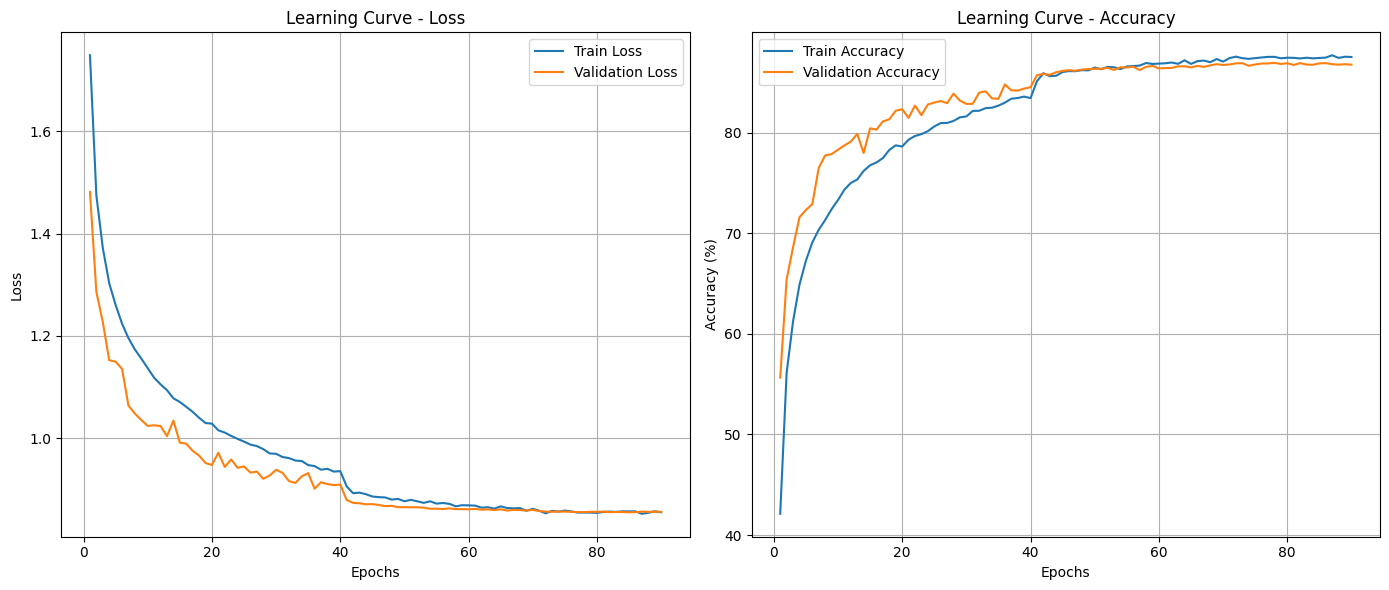
\includegraphics[width=0.9\textwidth]{learning_curves.png}
     \caption{Learning Curves (Loss and Accuracy).} % Translated
     \label{fig:learning_curves}
 \end{figure}
 In the first 40 epochs, both train loss and validation loss decreased synchronously, indicating that the model was learning useful features. Afterward, slight signs of overfitting appeared as train loss continued to decrease while validation loss fluctuated around 0.85-0.90.

 Validation accuracy stabilized at 86-87\% from epochs 40-50, while train accuracy continued to rise to nearly 90\%. Although there was slight overfitting, thanks to regularization techniques like Dropout, Weight Decay, Label Smoothing, and data augmentation, the model still maintained good generalization ability.

 \section{Performance on the Test Set} % Translated
 \textbf{Overall Results} % Translated

 The model achieved 86.80\% accuracy on the test set, very close to the validation accuracy (86.89\%), with only a 0.09\% difference. This consistency shows that the model was not severely overfitted and has good generalization ability.

 \textbf{Class-wise Performance} % Translated
 \begin{table}[H]
     \centering
     \caption{Class-wise accuracy on the test set} % Translated
     \begin{tabular}{lc}
         \toprule
         \textbf{Class} & \textbf{Accuracy (\%)} \\ % Translated
         \midrule
         Car & 94.3 \\
         Ship & 93.0 \\
         Truck & 92.0 \\
         Horse & 89.9 \\
         Frog & 89.3 \\
         Plane & 89.0 \\
         Deer & 85.7 \\
         Dog & 81.3 \\
         Bird & 80.2 \\
         Cat & 73.3 \\
         \bottomrule
     \end{tabular}
     \label{tab:class_accuracy}
 \end{table}
 The leading group consists of vehicles (car, ship, truck) with accuracy above 92\%. These objects have distinct characteristic shapes and fewer variations, making them easy to distinguish from other classes. The more challenging group is animals, especially the trio of cat, bird, and dog. The reason is the great diversity in posture, viewpoint, and color within the same class, and many common features among species.

 \section{Confusion Matrix Analysis} % Translated
 \begin{figure}[H]
     \centering
     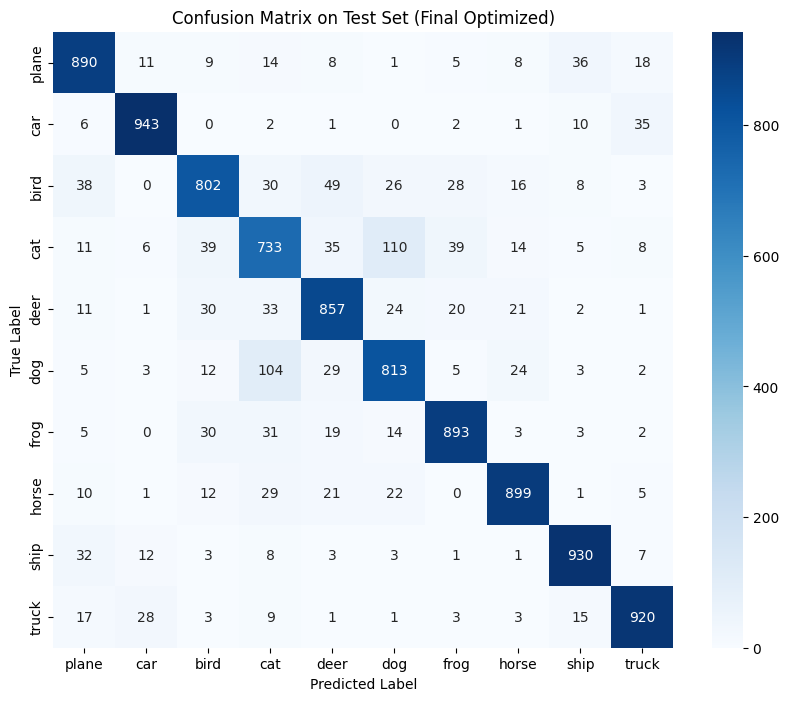
\includegraphics[width=0.7\textwidth]{confusion_matrix.png}
     \caption{Confusion matrix on the test set.} % Translated
     \label{fig:confusion_matrix}
 \end{figure}
 Main confusion pairs:
 \begin{itemize}
     \item cat $\leftrightarrow$ dog: 214 cases (110 + 104) - the most confused pair % Translated
     \item bird $\rightarrow$ deer: 49 cases % Translated
     \item deer $\rightarrow$ cat: 33 cases % Translated
     \item bird $\rightarrow$ cat: 30 cases % Translated
 \end{itemize}

 The cat-dog pair being the most confused is understandable as both are four-legged animals with fur and pointed ears. In the 32x32 pixel space of CIFAR-10, subtle distinguishing details can be lost. Bird appears in several different confusion pairs, suggesting that in the feature space learned by the model, some bird images share common characteristics with other animals at certain viewing angles.

 \section{Overall Assessment} % Translated
 After the training and evaluation process, the Convolutional Neural Network (CNN) model has demonstrated significant performance on the CIFAR-10 dataset, achieving an overall accuracy of 86.80\% on the test set. This result reflects the success in integrating modern training techniques such as diverse data augmentation, effective regularization methods, along with mechanisms for automatic learning rate adjustment and early stopping. The model has proven its good generalization ability, evidenced by the consistency between performance on the validation and test sets, while also showing superior performance in classifying object classes with clear visual features such as vehicles ('car', 'ship', 'truck').

 However, after a detailed analysis of the results, I also recognized some limitations. Slight overfitting is still observable through the learning curves, indicating a need for further improvement in generalization ability. Furthermore, the model encountered more difficulty in distinguishing animal classes with high visual similarity (e.g., 'cat' and 'dog'), with significantly lower accuracy compared to other classes. This suggests that the current 3-layer CNN architecture, while effective, may not be sufficiently capable of capturing the subtle differences between these complex classes.

 Thus, the current CNN model that I have built is a solid foundation, demonstrating success in applying deep learning principles. The analyses of strengths and limitations that I performed not only affirm what the CNN model has achieved but also help me outline a clear roadmap for future optimization and performance enhancement steps. This will guide me towards more effectively addressing the remaining challenges in complex image classification tasks, especially with objects that have high visual similarities, such as animal species.

 \end{document}